\documentclass{article}

\usepackage[version=3]{mhchem}
\usepackage{siunitx}
\usepackage{natbib}
\usepackage{graphicx}
\usepackage{mathtools}
\usepackage{amssymb}
\usepackage{amsthm}
\usepackage[italian]{babel}
\usepackage{stackengine}
\usepackage{graphicx,ifthen}
\usepackage{amsmath}
\usepackage{hyperref}
\usepackage{upgreek}
\usepackage{bm}

\renewcommand{\labelenumi}{\alph{enumi}.} % Make numbering in the enumerate environment by letter rather than number (e.g. section 6)

\title{Esperienza V: \\ banco ottico}
\author{Manuel G. Moretti\footnote{email: manuel.moretti560@edu.unito.it}}
\date{Luglio 2024}

\begin{document}

\maketitle

\begin{center}
\begin{tabular}{l r}
Esperimentazioni II corso B & A.A. 2023/24 \\
Modulo II & Universit\'{a} degli Studi di Torino \\
\end{tabular}
\end{center}

\begin{abstract}
In questa esperienza si è stimata la lunghezza focale di una lente biconvessa e di una lente biconcava facendo uso della legge dei punti coniugati. Inoltre, si è verificata la legge dell'ingrandimento per una lente convergente.
\end{abstract}

\section{Obiettivi della misura}
Gli obiettivi di questa esperienza sono due. Il primo consiste nello stimare la lunghezza focale di una lente biconvessa e di una lente biconcava tramite la legge dei punti coniugati, la quale mette in relazione la distanza focale $f$ con le distanze lente-oggetto, $p$, e lente-schermo, $q$, secondo l'equazione
\begin{equation}
    \label{eq:legge punti coniugati}
    \frac{1}{p}+\frac{1}{q}=\frac{1}{f}.
\end{equation}
Il secondo obiettivo invece riguarda la verifica della legge di ingrandimento per una lente convergente
\begin{equation}
    \label{eq:legge ingrandimento}
    G=\frac{q}{p}.
\end{equation}
\section{Configurazione dell'apparato sperimentale}
L'apparato sperimentale consiste in un banco ottico, ovvero una rotaia graduata, sul quale vengono posizionati, in quest'ordine, una lampada, una diapositiva sulla quale è impressa un semplice disegno geometrico, il sostegno per le lenti e uno schermo sul quale l'immagine viene proiettata.

\section{Raccolta ed elaborazione dei dati}
\subsection{Stima della distanza focale}
Dopo aver posizionato sull'apposito sostegno la lente biconvessa ad una distanza $p=(122\pm1)$ mm, come passo preliminare di questa parte dell'esperienza, si sono raccolte cinquanta misure della distanza $q$ alla quale l'immagine proiettata sullo schermo risultasse a fuoco. Il medesimo procedimento si è ripetuto, dopo aver ruotato la lente di 180°, al fine di verificare che le misure di $q$ non dipendano dall'orientazione della lente, ovvero che quest'ultima sia simmetrica.

Dal primo set di dati ottenuto si è costruito un istogramma delle frequenze dei valori di $q$.
\begin{figure}[h]
    \centering
    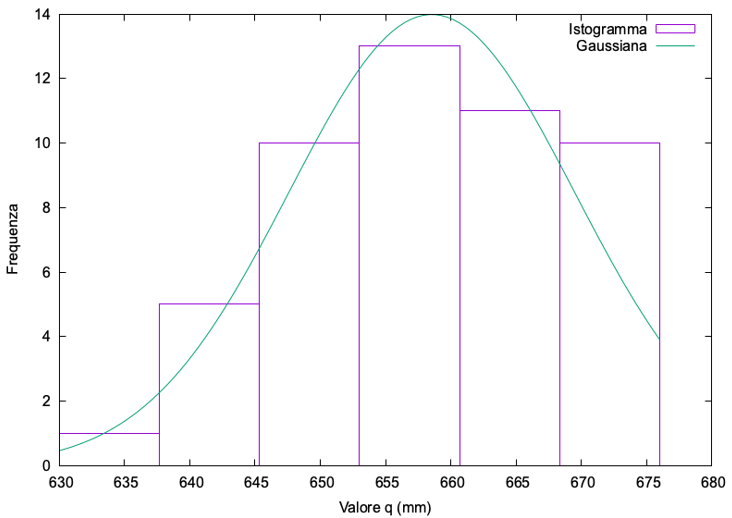
\includegraphics[width=0.4\linewidth]{Immagini/distribuzione.png}
    \caption{distribuzione dei valori di $q$}
    \label{fig:distribuzione q}
\end{figure}

Dai risultati della regressione si ottiene che la distribuzione è compatibile con una gaussiana ad un livello di significatività del 5\% ($\chi^2=2.31$ e $DOF=3$). Si osservi inoltre come il valore medio delle misure di $q$ del primo set di dati sia compatibile con quello del secondo set, rispettivamente $(658.54\pm10.93)$ mm e $(653.64\pm8.75)$ mm, confermando così che la lente sia simmetrica. 

L'esperienza prosegue, sempre con la lente biconvessa, con la raccolta di sei set di dati, dove in ognuno di questi si è fissata una distanza $p$ e si è misurata sei volte la distanza $q$ alla quale l'immagine sullo schermo risultasse a fuoco. Con i dati raccolti da questo procedimento si è creato un grafico avente come ascisse i reciproci di $p$ e come ordinate i reciproci dei valori medi di $q$ di ogni set.
\begin{figure}[h]
    \centering
    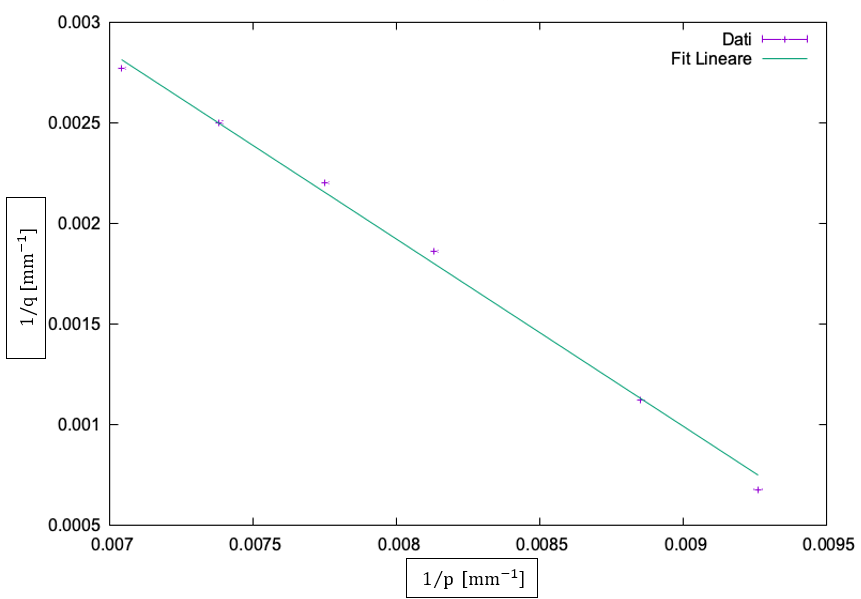
\includegraphics[width=0.45\linewidth]{Immagini/I fit.png}
    \caption{grafico di $q^{-1}(p^{-1})$ (lente biconvessa)}
    \label{fig:I fit}
\end{figure}
\newpage
Il medesimo procedimento si è ripetuto con l'aggiunta di una lente biconcava alla lente biconvessa. Con i dati raccolti si è creato un grafico analogo al quello in figura \ref{fig:I fit}.
\begin{figure}[h]
    \centering
    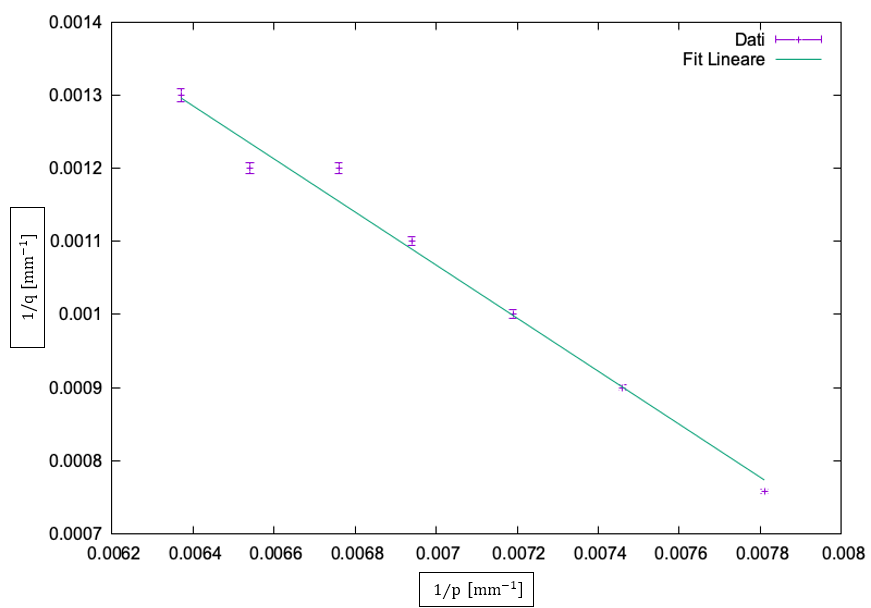
\includegraphics[width=0.5\linewidth]{Immagini/II fit.png}
    \caption{grafico di $q^{-1}(p^{-1})$ (sistema di lenti)}
    \label{fig:II fit}
\end{figure}


\subsection{Verifica della legge d'ingrandimento}
Per questa parte di esperienza la raccolta dati è consistita in sei coppie di misure di $p$ e $q$, dove per ognuna veniva misurata tramite un calibro la dimensione di un particolare di lunghezza  mm dell'immagine sulla diapositiva $d=(6.6\pm1.0)$, la quale veniva proiettata sullo schermo. I dati ottenuti sono raccolti nella seguente tabella.
% Requires: \usepackage{graphicx}
\begin{table}[h]
 \centering
 \begin{tabular}{|c|c|c|c|}
  \hline
  \textbf{p [mm]} & \textbf{q [mm]} & \bm{$G_{mis}$} & \bm{$G_{calc}$} \\ \hline
  $108\pm1$ & $1480.0\pm5.3$ & $13.79\pm0.26$ & $13.70\pm0.14$ \\ \hline
  $129\pm1$ & $455.0\pm5.3$  & $3.49\pm0.16$ & $3.52\pm0.05$ \\ \hline
  $142\pm1$ & $361.0\pm5.3$  & $2.58\pm0.16$ & $2.54\pm0.04$ \\ \hline
  $135\pm1$ & $400.0\pm5.3$  & $3.03\pm0.16$ & $2.95\pm0.05$ \\ \hline
  $123\pm1$ & $536.0\pm5.3$  & $4.10\pm0.16$ & $4.36\pm0.06$ \\ \hline
  $113\pm1$ & $892.0\pm5.3$  & $7.89\pm0.19$ & $7.90\pm0.08$  \\ \hline
 \end{tabular}
 \caption{misure di $p$, $q$, $G_{mis}$ e $G_{calc}$}
 \label{tab:misure di p q G}
\end{table}

Nella quale $G_{mis}$ si riferisce al valore di $G$ calcolato a partire dalle misure effettuate con il calibro e $G_{calc}$ si riferisce a quello calcolato a partire dalle misure di $p$ e $q$.

\newpage
\section{Risultati e conclusioni}
Dal primo set di dati, ottenuto durante il passo preliminare della prima parte di esperienza, calcolando il valore medio di $q=(658.54\pm10.93)$ e sfruttando l'equazione \eqref{eq:legge punti coniugati}, si ottiene un valore della focale $f_{conv}^{(1)}$ della lente biconvessa di $f_{conv}^{(1)}=(102.93\pm2.01)$ mm.

Usando il reciproco dell'intercetta $a_1$ della retta ottenuta dalla regressione lineare effettuata sul grafico in figura \ref{fig:I fit}, $a_1=(0.0094\pm0.0010)$ mm$^{-1}$, è stato possibile determinare il valore della lunghezza focale $f_{conv}$ della stessa lente biconvessa ottenendo $f_{conv}^{(2)}=(106.48\pm2.20)$ mm. Si noti come effettuando un test di Gauss tra i valori della focale $f_{conv}^{(1)}$ e $f_{conv}^{(2)}$ si ottenga un valore di $Z$ di $Z=1.32$, il quale è minore del valore critico di $1.96$. Pertanto, le due misure della focale della lente biconvessa risultano statisticamente compatibili ad un livello di significatività del 5\%. Analogamente, dall'intercetta $a_2$ della retta ottenuta dalla regressione dei dati rappresentati nel grafico in figura \ref{fig:II fit}, $a_2=(0.0036\pm0.0010)$ mm$^{-1}$, si è stimata la lunghezza focale $f_{sist}$ del sistema di lenti sottili, formato dalla lente biconvessa e da quella biconcava. Infatti, usando la formula della focale per sistemi di legge sottili
\begin{equation}
    \label{eq:focale sistemi}
    \frac{1}{f_{sist}}=\frac{1}{f_{conc}}+\frac{1}{f_{conv}},
\end{equation}
si è ottenuto $f_{conc}=(-169.49\pm28.73)$ mm, dove come valore di $f_{conv}$ si è usata la media di $f_{conv}^{(1)}$ e $f_{conv}^{(2)}$, ovvero $f_{conv}=(104.86\pm2.11)$ mm. Il valore di $f_{conc}$ è compatibile con il fatto che la lente biconcava è una lente divergente, quindi la sua focale è negativa. 

Dai dati raccolti in tabella \ref{tab:misure di p q G} è ora possibile effettuare dei test di Gauss tra i rispettivi valori di $G_{mis}$ e $G_{calc}$. Questi ultimi restituiscono dei valori di $Z$ minori del valore critico di $1.96$. Dunque le stime di $G_{mis}$ e $G_{calc}$ sono statisticamente compatibili ad un livello di significatività del 5\%, verificando pertanto la legge dell'ingrandimento enunciata con l'equazione \eqref{eq:legge ingrandimento}.

\end{document}